\documentclass[a4paper,12pt]{article}
\usepackage [catalan] {babel} 
\usepackage [latin1]{inputenc}
\usepackage{setspace}
\usepackage{graphicx}
\onehalfspacing

\begin{document}
\title{\textbf{PAC3 Control de Versions i Documentaci�}}
\author{Alfredo Rafael Vicente Boix}
\date{15 de desembre de 2015}
\maketitle
\pagebreak
\part*{Introducci�}

Aquest document presenta les 3 parts de la pr�ctica realitzada de l'assignatura Desenvolupament de Programari de la Universitat Oberta de Catalunya. El document est� format per dues parts on s'explica el proc�s i els pasos a seguir per resoldre els diferents problemes.\\
Al primer problema s'ha utilitzat la ferramenta git per a crear el repositori i guthub per a compartirlo.\\
El segon problema s'han utilitzat les etiquetes doxygen i el programa doxywizard per a poder formatar la documentaci� amb html.\\


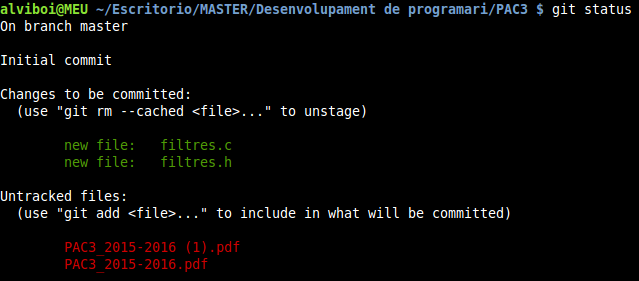
\includegraphics[width=\linewidth]{./images/pic1.png}
\pagebreak
\part*{Control de Versions}
\paragraph{}


\section{Documentaci�}

\section{Conclusions}


\end{document}